\subsection{Multiple Integration and Change of Variables}

% **Role:** calculus as local linearization plus global geometric integration.
%
% Alternating forms, pullbacks, orientation, manifolds, integration on manifolds.

This subsection moves from Euclidean-region integration and change of variables to differential forms, pullbacks, and oriented parametrized surfaces.

\begin{theorem} \label{thm:linear-map-volume-scaling-determinant} \hlt{Linear Maps Scale Volume by $\abs{\det T}$}\\
Let $T\in\LL(\mathbb{R}^n)$ and let $\Omega\subseteq\mathbb{R}^n$ be bounded Jordan measurable.
\begin{enumerate}[label=(\roman*)]
\setlength{\itemsep}{0pt}
\item $T(\Omega)$ is Jordan measurable.
\item $\operatorname{vol}(T(\Omega))=\abs{\det T}\operatorname{vol}(\Omega)$.
\end{enumerate}
\begin{proof}
If $T$ invertible, let $T=SP$ with $S$ orthogonal, $P=\operatorname{diag}(\lambda_1,\ldots,\lambda_n)$, $\lambda_j>0$, in orthonormal coordinates.
\begin{enumerate}[label=(\roman*)]
\setlength{\itemsep}{0pt}
\item If $T$ is invertible, $P$ and $S$ preserve Jordan measurability, so $T(\Omega)$ is Jordan measurable.\\
If $T$ is singular, $T(\Omega)\subseteq W$ for a proper affine subspace $W$, hence $T(\Omega)$ is Jordan null.
\item If $T$ is invertible, rectangle scaling gives $\operatorname{vol}(P\Omega)=(\det P)\operatorname{vol}(\Omega)$ by Jordan approximation.\\
Hhence $\operatorname{vol}(T\Omega)=\operatorname{vol}(P\Omega)=\abs{\det T}\operatorname{vol}(\Omega)$. If $T$ is singular, (i) gives $\operatorname{vol}(T\Omega)=0=\abs{\det T}\operatorname{vol}(\Omega)$.
\end{enumerate}
\hlt{Structural Commentary}: Polar decomposition leaves only diagonal stretching.\\
\hlt{Key Insight}: $\abs{\det T}$ is total coordinate stretch.
\end{proof}
\end{theorem}

\begin{figure}[H]
  \centering
  \begin{tikzpicture}[
  >=Stealth,
  every node/.style={font=\small},
  axis/.style={->, gray!70},
  vec/.style={->, line width=1pt},
  areaA/.style={fill=blue!12, draw=blue!50},
  areaB/.style={fill=red!12, draw=red!55},
  arrow/.style={->, line width=0.85pt, blue!70!black}
]
  \begin{scope}
    \draw[axis] (-0.2,0) -- (2.4,0);
    \draw[axis] (0,-0.2) -- (0,2.0);
    \draw[areaA] (0,0) rectangle (1.35,1.05);
    \node at (0.68,0.52) {$\Omega$};
  \end{scope}

  \draw[arrow] (2.7,0.75) -- (4.1,0.75) node[midway, above=4pt] {$T$};

  \begin{scope}[shift={(4.5,0)}]
    \draw[axis] (-0.2,0) -- (3.0,0);
    \draw[axis] (0,-0.2) -- (0,2.2);
    \coordinate (O) at (0,0);
    \coordinate (a) at (2.25,0.35);
    \coordinate (b) at (0.65,1.55);
    \coordinate (ab) at ($(a)+(b)$);
    \draw[areaB] (O) -- (a) -- (ab) -- (b) -- cycle;
    \draw[vec, blue!75!black] (O) -- (a);
    \draw[vec, red!75!black] (O) -- (b);
    \node at (1.45,0.95) {$T(\Omega)$};
  \end{scope}
\end{tikzpicture}

  \caption{A linear map scales volume by $\abs{\det T}$.}
  \label{fig:determinant-volume-scaling}
\end{figure}

\begin{definition} \label{def:multiple-integration-core-source-todo}\label{def:k-cell-and-multiple-integral} \hlt{$k$-Cells and Multiple Integrals}\\
Let $a_i\leq b_i$.
\begin{enumerate}[label=(\roman*)]
\setlength{\itemsep}{0pt}
\item Set $I^j\defeq\prod\limits_{i=1}^{j}[a_i,b_i]\subseteq\R^j$ for $0\leq j\leq k$, with $I^0$ a point. The \hlt{$k$-cell} is $I^k$.
\item For $f\in C(I^k)$, set $f_k\defeq f$ and $f_{j-1}(x_1,\ldots,x_{j-1})\defeq\int_{a_j}^{b_j}f_j(x_1,\ldots,x_j)\,dx_j$, $j=k,\ldots,1$.\\
The \hlt{multiple integral} is $\int_{I^k}f(\x)\,d\x\defeq f_0$, also written $\int_{I^k}f$.
\end{enumerate}
\end{definition}

For bounded functions on rectangles, the Darboux picture from Definition \ref{def:partition-and-riemann-upper-lower-sums} generalizes by replacing intervals with grid rectangles.

\begin{definition} \label{def:rectangular-grid-riemann-sum} \hlt{Rectangular Grids and Riemann Sums}\\
Let $R=[a,b]\times[c,d]\subseteq\R^2$, let $P:a=x_0<\cdots<x_m=b$, let $Q:c=y_0<\cdots<y_n=d$, and set $G\defeq P\times Q$.
\begin{enumerate}[label=(\roman*)]
\setlength{\itemsep}{0pt}
\item The \hlt{grid rectangles} are $R_{ij}\defeq[x_{i-1},x_i]\times[y_{j-1},y_j]$, with $\abs{R_{ij}}\defeq(x_i-x_{i-1})(y_j-y_{j-1})$.
\item For tags $S=\{(s_{ij},t_{ij})\in R_{ij}\}$, the \hlt{Riemann sum} is $R(f,G,S)\defeq\sum\limits_{i=1}^{m}\sum\limits_{j=1}^{n}f(s_{ij},t_{ij})\abs{R_{ij}}$.
\item For bounded $f:R\to\R$, set $(m_{ij},M_{ij})\defeq(\inf_{R_{ij}}f,\sup_{R_{ij}}f)$ and $(L(f,G),U(f,G))\defeq\sum\limits_{i,j}(m_{ij},M_{ij})\abs{R_{ij}}$.
\item The \hlt{lower} and \hlt{upper integrals} are $\underline{\int_R}f\defeq\sup_G L(f,G)$ and $\overline{\int_R}f\defeq\inf_G U(f,G)$.\\
If they agree, $f$ is Riemann integrable on $R$, and $\int_R f$ denotes the common value.
\end{enumerate}
\end{definition}

\begin{figure}[H]
  \centering
  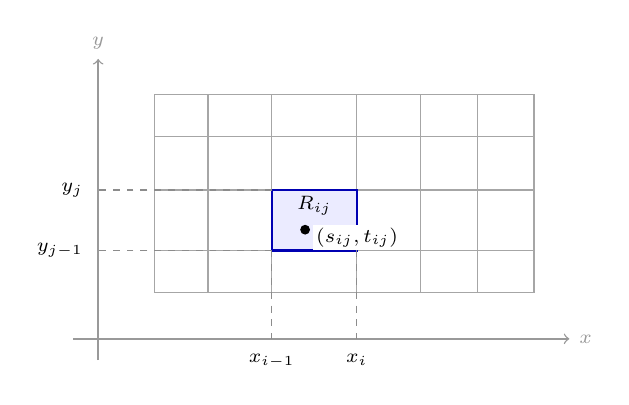
\begin{tikzpicture}[
  scale=0.9,
  every node/.style={font=\scriptsize},
  gridline/.style={black!35, line width=0.45pt},
  axis/.style={->, black!40, line width=0.5pt},
  cell/.style={fill=blue!8, draw=blue!70!black, line width=0.9pt},
  point/.style={circle, fill=black, inner sep=1.25pt},
  guide/.style={black!45, dashed, dash pattern=on 2.5pt off 2.5pt, line width=0.45pt}
]
  \draw[axis] (-0.35,0) -- (6.65,0) node[right] {$x$};
  \draw[axis] (0,-0.30) -- (0,3.95) node[above] {$y$};

  \foreach \x in {0.80,1.55,2.45,3.65,4.55,5.35,6.15} {
    \draw[gridline] (\x,0.65) -- (\x,3.45);
  }
  \foreach \y in {0.65,1.25,2.10,2.85,3.45} {
    \draw[gridline] (0.80,\y) -- (6.15,\y);
  }

  \draw[cell] (2.45,1.25) rectangle (3.65,2.10);
  \node at (3.05,1.88) {$R_{ij}$};
  \node[point] at (2.92,1.54) {};
  \node[fill=white, inner sep=1pt, anchor=west] at (3.03,1.43) {$(s_{ij},t_{ij})$};

  \draw[guide] (2.45,1.25) -- (2.45,0);
  \draw[guide] (3.65,1.25) -- (3.65,0);
  \draw[guide] (2.45,1.25) -- (0,1.25);
  \draw[guide] (2.45,2.1) -- (0,2.1);

  \node[below=2pt] at (2.45,0) {$x_{i-1}$};
  \node[below=2pt] at (3.65,0) {$x_i$};
  \node[left=2pt] at (0,1.25) {$y_{j-1}$};
  \node[left=2pt] at (0,2.1) {$y_j$};
\end{tikzpicture}

  \caption{A grid rectangle $R_{ij}$ and sample point $(s_{ij},t_{ij})$.}
  \label{fig:riemann-grid-sample-rectangle}
\end{figure}

\begin{theorem} \label{thm:fubini-riemann-rectangle-slices} \hlt{Fubini on a Rectangle, Darboux Form}\\
Let $R=[a,b]\times[c,d]$, let $f:R\to\R$ be Riemann integrable, and set $f_y(x)\defeq f(x,y)$.\\
For $y\in[c,d]$, define $\underline{F}(y)\defeq\sup_P L(P,f_y)$ and $\overline{F}(y)\defeq\inf_P U(P,f_y)$, with $P$ ranging over partitions of $[a,b]$.
\begin{enumerate}[label=(\roman*)]
\setlength{\itemsep}{0pt}
\item $\underline{F},\overline{F}$ are Riemann integrable on $[c,d]$.
\item $\int_R f=\int_c^d\underline{F}(y)\,dy=\int_c^d\overline{F}(y)\,dy$.
\end{enumerate}
If $\int_a^b f(x,y)\,dx$ exists for every $y$, then $\underline{F}(y)=\overline{F}(y)=\int_a^b f(x,y)\,dx$.
\begin{proof}
\begin{enumerate}[label=(\roman*)]
\setlength{\itemsep}{0pt}
\item For $G=P\times Q$, horizontal slice sums give $L(f,G)\leq L(Q,\underline{F})\leq U(Q,\overline{F})\leq U(f,G)$.\\
Since $f$ is integrable on $R$, choose $G$ with $U(f,G)-L(f,G)<\varepsilon$; hence $U(Q,\overline{F})-L(Q,\underline{F})<\varepsilon$.\\
Thus $\underline{F}$ and $\overline{F}$ are integrable and have the same integral by Theorem \ref{thm:riemann-stieltjes-integrability-criterion}.
\item The same inequalities give $L(f,G)\leq\int_c^d\underline{F}\leq\int_c^d\overline{F}\leq U(f,G)$.\\
Letting $U(f,G)-L(f,G)\to0$ gives both integrals equal to $\int_R f$.
\end{enumerate}
\hlt{Structural Commentary}: Product grids become slice sums.\\
\hlt{Key Insight}: Fubini is a Darboux squeeze.
\end{proof}
\end{theorem}

\begin{theorem} \label{thm:iterated-integrals-order-independent} \hlt{Order Independence on Cells}\\
For $f\in C(I^k)$, all iterated orders defining $\int_{I^k}f$ give the same value.
\begin{proof}
Let $L,L'$ be two iterated orders. For $h(\x)=h_1(x_1)\cdots h_k(x_k)$, $L(h)=L'(h)=\prod\limits_{i=1}^k\int_{a_i}^{b_i}h_i(x_i)\,dx_i$, so $L(g)=L'(g)$ for every finite sum $g$ of such products. These sums are dense in $C(I^k)$ by Theorem \ref{thm:real-stone-weierstrass}.\\
Choose $g$ with $\norm{f-g}_\infty<\varepsilon/V$, where $V=\prod\limits_{i=1}^k(b_i-a_i)$.\\
Since $\abs{L(r)},\abs{L'(r)}\leq V\norm{r}_\infty$, then $\abs{L(f)-L'(f)}\leq\abs{L(f-g)}+\abs{L'(f-g)}<2\varepsilon$.\\
\hlt{Structural Commentary}: Product functions plus uniform approximation prove order independence.\\
\hlt{Key Insight}: Fubini-type order independence is first an algebraic fact, then a uniform approximation fact.
\end{proof}
\end{theorem}

\begin{perspective} \label{per:fubini-hypotheses-control-order} \hlt{Order Interchange Requires Hypotheses}\\
Finite sums are order-free; limiting processes are not.\\
Theorems \ref{thm:fubini-riemann-rectangle-slices} and \ref{thm:iterated-integrals-order-independent} give hypotheses for interchanging integral order.
\end{perspective}

\begin{definition} \label{def:support-and-compact-support-integral} \hlt{Support and Simplex Integrals}\\
For $f:\R^k\to\R$ or $\C$, define $\operatorname{supp}f\defeq\overline{\{\x\in\R^k:f(\x)\neq0\}}$.
\begin{enumerate}[label=(\roman*)]
\setlength{\itemsep}{0pt}
\item For $f\in C_c(\R^k)$ and any cell $I^k\supseteq\operatorname{supp}f$, define $\int_{\R^k}f\defeq\int_{I^k}f$; this is independent of $I^k$.
\item The \hlt{standard $k$-simplex} is $Q^k\defeq\{\x\in\R^k:x_i\geq0,\ \sum\limits_{i=1}^{k}x_i\leq1\}$.\\
For $f\in C(Q^k)$, extend $f$ by $0$ to $[0,1]^k$ and define $\int_{Q^k}f$ as the corresponding multiple integral.
\end{enumerate}
\end{definition}

\begin{definition} \label{def:primitive-mapping-and-flip} \hlt{Primitive Mappings and Flips}\\
Let $E\subseteq\R^n$ be open.
\begin{enumerate}[label=(\roman*)]
\setlength{\itemsep}{0pt}
\item $G:E\to\R^n$ is \hlt{primitive in coordinate $m$} if $G(\x)=(x_1,\ldots,x_{m-1},g(\x),x_{m+1},\ldots,x_n)$.
\item If $g$ is differentiable at $\a\in E$, then $DG(\a)$ is $I_n$ except row $m$ is $\nabla g(\a)$, and $J_G(\a)=(D_mg)(\a)$.
\item A \hlt{flip} is a linear map $B:\R^n\to\R^n$ with $B\mathbf{e}_p=\mathbf{e}_q$, $B\mathbf{e}_q=\mathbf{e}_p$, and $B\mathbf{e}_i=\mathbf{e}_i$ for $i\notin\{p,q\}$, $p\neq q$.
\end{enumerate}
\end{definition}

\begin{theorem} \label{thm:local-decomposition-primitive-mappings} \hlt{Local Decomposition into Primitive Mappings}\\
Let $E\subseteq\R^n$ be open, let $\F\in C^1(E,\R^n)$, let $\ze\in E$, and assume $\F(\ze)=\ze$ and $D\F(\ze)$ is invertible. Then there exist a neighborhood $U$ of $\ze$, primitive $C^1$ maps $G_1,\ldots,G_n$ near $\ze$, and maps $B_1,\ldots,B_{n-1}$ such that:
\begin{enumerate}[label=(\roman*)]
\setlength{\itemsep}{0pt}
\item $G_i(\ze)=\ze$, $DG_i(\ze)$ is invertible, and each $B_i$ is a flip or $I$.
\item $\F=B_1\cdots B_{n-1}G_n\circ\cdots\circ G_1$ on $U$.
\end{enumerate}
\begin{proof}
Let $P_m\x\defeq\sum\limits_{i=1}^{m}x_i\mathbf{e}_i$ and set $\F_1\defeq\F$.
\begin{enumerate}[label=(\roman*)]
\setlength{\itemsep}{0pt}
\item Suppose $P_{m-1}\F_m=P_{m-1}$, $\F_m(\ze)=\ze$, and $D\F_m(\ze)$ invertible, and write $\F_m=P_{m-1}+\sum\limits_{i=m}^{n}\alpha_i\mathbf{e}_i$.\\
Choose $k\geq m$ with $(D_m\alpha_k)(\ze)\neq0$, let $B_m$ swap $m,k$ (or $B_m=I$), set $G_m(\x)\defeq\x+(\alpha_k(\x)-x_m)\mathbf{e}_m$.\\
Then $G_m$ is primitive, $G_m(\ze)=\ze$, $J_{G_m}(\ze)\neq0$, and $G_m$ is locally invertible.\\
With $\F_{m+1}\defeq B_m\F_m\circ G_m^{-1}$, one has $P_m\F_{m+1}=P_m$, $\F_{m+1}(\ze)=\ze$, and $D\F_{m+1}(\ze)$ invertible.\\
Iterate for $m=1,\ldots,n-1$ and set $G_n\defeq\F_n$.
\item From $\F_{m+1}=B_m\F_m\circ G_m^{-1}$ and $B_m^2=I$, $\F_m=B_m\F_{m+1}\circ G_m$.\\
Iteration gives $\F=\F_1=B_1\cdots B_{n-1}G_n\circ G_{n-1}\circ\cdots\circ G_1$ near $\ze$.
\end{enumerate}
\hlt{Structural Commentary}: Local diffeomorphisms factor by coordinate elimination.\\
\hlt{Key Insight}: Nonlinear elimination follows $D\F(\ze)$.
\end{proof}
\end{theorem}

\begin{theorem} \label{thm:partition-of-unity-rudin} \hlt{Partition of Unity on a Compact Set}\\
Let $K\subseteq\R^n$ be compact and let $\{V_\alpha\}$ cover $K$ by open sets. Then there are $\psi_1,\ldots,\psi_s\in C^1(\R^n)$ such that
\begin{enumerate}[label=(\roman*)]
\setlength{\itemsep}{0pt}
\item $0\leq\psi_i\leq1$ for all $i$;
\item $\operatorname{supp}(\psi_i)\subseteq V_\alpha$ for some $\alpha$;
\item $\sum_{i=1}^s\psi_i=1$ on $K$.
\end{enumerate}
If $f\in C(\R^n)$ and $\operatorname{supp}(f)\subseteq K$, then $f=\sum_{i=1}^{s}\psi_if$, with each summand supported in one member of the cover.
\begin{proof}
\begin{enumerate}[label=(\roman*)]
\setlength{\itemsep}{0pt}
\item For each $\x\in K$, choose balls with $\overline{B(\x)}\subseteq W(\x)\subseteq\overline{W(\x)}\subseteq V_{\alpha(\x)}$.\\
By compactness, Definition \ref{def:open-cover-and-compactness}, finitely many $B(\x_i)$ cover $K$.
\item Choose $\varphi_i\in C^1(\R^n)$ with $\varphi_i=1$ on $B(\x_i)$ and $\operatorname{supp}(\varphi_i)\subseteq W(\x_i)$. Set $\psi_i=(1-\varphi_1)\cdots(1-\varphi_{i-1})\varphi_i$.
\item Then $0\leq\psi_i\leq1$, each $\psi_i$ is supported in some $V_\alpha$, and $\sum\limits_{i=1}^{s}\psi_i=1-\prod\limits_{i=1}^{s}(1-\varphi_i)$, which equals $1$ on $K$.\\
Multiplying by $f$ gives the final assertion.
\end{enumerate}
\hlt{Structural Commentary}: Compactness finite; product cutoffs sum to one.\\
\hlt{Key Insight}: A partition of unity turns local change-of-variable information into a global formula.
\end{proof}
\end{theorem}

The nonlinear change-of-variables theorem is the local volume-scaling formula from Theorem \ref{thm:linear-map-volume-scaling-determinant} applied cell by cell after a fine grid has been warped by a $C^1$ diffeomorphism.

\begin{figure}[H]
  \centering
  \begin{tikzpicture}[
  scale=0.85,
  >=Stealth,
  every node/.style={font=\scriptsize},
  gridline/.style={black!35, line width=0.45pt},
  boundary/.style={black!60, line width=0.75pt},
  warp/.style={blue!70!black, line width=0.55pt},
  arrow/.style={->, line width=0.8pt},
  region/.style={fill=blue!5, draw=black!60, line width=0.75pt}
]
  \begin{scope}
    \draw[region] (0,0) rectangle (3,3);
    \foreach \x in {0.6,1.2,1.8,2.4} {
      \draw[gridline] (\x,0.35) -- (\x,2.65);
    }
    \foreach \y in {0.6,1.2,1.8,2.4} {
      \draw[gridline] (0.35,\y) -- (2.65,\y);
    }
    \node[below=3pt] at (1.5,0) {$U$};
  \end{scope}

  \draw[arrow] (3.55,1.5) -- node[above=2pt] {$T$} (4.65,1.5);

  \begin{scope}[xshift=5.05cm]
    \draw[boundary, fill=blue!5]
      (0.10,0.35)
      .. controls (0.95,0.05) and (2.45,0.10) .. (3.35,0.32)
      .. controls (3.55,1.05) and (3.50,2.15) .. (3.25,2.92)
      .. controls (2.25,3.22) and (0.95,3.18) .. (0.25,2.90)
      .. controls (-0.05,2.15) and (-0.08,1.05) .. (0.10,0.35);

    \foreach \x in {0.70,1.25,1.80,2.35,2.90} {
      \draw[warp]
        (\x,0.42)
        .. controls (\x-0.18,1.05) and (\x+0.18,2.00) ..
        (\x+0.05,2.82);
    }
    \foreach \y in {0.72,1.18,1.64,2.10,2.56} {
      \draw[warp]
        (0.25,\y)
        .. controls (1.05,\y+0.12) and (2.30,\y-0.10) ..
        (3.20,\y+0.05);
    }

    \node[blue!70!black, fill=blue!5, inner sep=1pt] at (2.45,2.40) {$\abs{J_T}$};
    \node[below=3pt] at (1.75,0.20) {$T(U)$};
  \end{scope}
\end{tikzpicture}

  \caption{A $C^1$ change of variables turns a fine grid into curvilinear cells; $\abs{J_T}$ records local volume scaling.}
  \label{fig:change-of-variables-grid-warp}
\end{figure}

\begin{theorem} \label{thm:change-of-variables-rk}\label{thm:multiple-integration-main-source-todo} \hlt{Change of Variables in $\R^k$}\\
Let $T:E\to\R^k$ be one-to-one and $C^1$ on open $E\subseteq\R^k$, with $J_T\neq0$ on $E$.\\
If $f\in C(\R^k)$ and $\operatorname{supp}(f)$ is compact in $T(E)$, then $\int_{\R^k}f(\y)\,d\y = \int_{\R^k}f(T(\x))\,\abs{J_T(\x)}\,d\x$.
\begin{proof}
Let $\mathcal{C}$ be the class of maps for which formula holds for all continuous functions with compact support in the image. Primitive maps lie in $\mathcal{C}$ by one-variable substitution, and flips lie in $\mathcal{C}$ by Theorem \ref{thm:iterated-integrals-order-independent}.\\
If $P,Q\in\mathcal{C}$, then $P\circ Q\in\mathcal{C}$, since Theorems \ref{thm:chain-rule-several-variables} and \ref{thm:determinant-basic-laws} give $J_{P\circ Q}(\x)=J_P(Q(\x))J_Q(\x)$.\\
After translating coordinates, Theorem \ref{thm:local-decomposition-primitive-mappings} therefore gives the formula on a neighborhood of each point of $E$. By Theorem \ref{thm:inverse-function-theorem-rn}, these neighborhoods have open images covering $\operatorname{supp}(f)$.\\
Choose a partition of unity from Theorem \ref{thm:partition-of-unity-rudin}, write $f=\sum_i\psi_i f$ with each $\psi_i f$ supported in one such image, apply the local formula to each summand, and sum.\\
\hlt{Structural Commentary}: Model cases plus partitions of unity prove the theorem.\\
\hlt{Key Insight}: The absolute Jacobian is local volume scaling, globalized by compact support.
\end{proof}
\end{theorem}

\begin{method} \label{meth:change-of-variables-jacobian} \hlt{Change-of-Variables Jacobian Method}\\
For a differentiable map $\sigma:\Omega\subseteq\mathbb{R}^n\to\mathbb{R}^n$:
\begin{enumerate}[label=(\roman*)]
\setlength{\itemsep}{0pt}
\item compute the derivative matrix $D\sigma(\mathbf{x})$;
\item compute the local volume factor $\abs{\det D\sigma(\mathbf{x})}$;
\item replace $d\mathbf{y}$ by $\abs{\det D\sigma(\mathbf{x})}\,d\mathbf{x}$ when $\mathbf{y}=\sigma(\mathbf{x})$;
\item transform the domain bounds in the new coordinates.
\end{enumerate}
\end{method}

\begin{example} \label{ex:polar-and-spherical-jacobians} \hlt{Polar and Spherical Jacobian Factors}\\
For polar coordinates $\sigma(r,\theta)=(r\cos\theta,r\sin\theta)$, $D\sigma(r,\theta)=
\begin{bmatrix}
\cos\theta & -r\sin\theta\\
\sin\theta & r\cos\theta
\end{bmatrix}$, and $\abs{\det D\sigma(r,\theta)}=r$.\\
Thus area integrals acquire the factor $r\,dr\,d\theta$.\\
For spherical coordinates $\sigma(\rho,\varphi,\theta) =(\rho\sin\varphi\cos\theta,\rho\sin\varphi\sin\theta,\rho\cos\varphi)$, and $\abs{\det D\sigma(\rho,\varphi,\theta)}=\rho^2\sin\varphi$.\\
Thus volume integrals acquire the factor $\rho^2\sin\varphi\,d\rho\,d\varphi\,d\theta$.
\end{example}

\begin{method} \label{meth:multiple-integration-proof-patterns-source-todo}\label{meth:multiple-integration-proof-patterns} \hlt{Multiple-Integration Proof Patterns}\\
For a multiple-integration identity:
\begin{enumerate}[label=(\roman*)]
\setlength{\itemsep}{0pt}
\item \hlt{Products}: prove product cases, then pass by uniform approximation;
\item \hlt{Grids}: compare product-grid upper and lower sums with one-variable slice sums;
\item \hlt{Support}: enclose compact support in a cell and check cell-independence;
\item \hlt{Local form}: reduce $C^1$ coordinate changes to primitive maps and flips;
\item \hlt{Determinants}: use multiplicativity and Theorem \ref{thm:determinant-basic-laws};
\item \hlt{Globalize}: apply the partition of unity, Theorem \ref{thm:partition-of-unity-rudin}.
\end{enumerate}
\hlt{Key Insight}: Change of variables is local determinant geometry plus compactness.
\end{method}
